\section{Supplementary material Section 1}

\subsection{Morphological characters states}
In order to obtain a realistic probabilistic value for of \textit{k} characters states for each simulated morphological character, we downloaded 100 random morphological characters (with more than 100 characters each) from TreeBASE database (http://treebase.org/) published between 1985 and 2013 and covering 19 taxomomic classess (Chordata, Arthropoda, Annelida, Angiosperm, Gymnosperm and Pteridophyta).
We selected a total of 22563 characters ranging from 2 to 10 states.
We calculated the proportion of characters with 2, 3, 4, 5, 6, 7, 8, 9 or 10 states.
We then sampeled 22563 \textit{k} values between 2 and 10 with the same proportion of characters from the empirical data.
We then used a simple t-test to check if our simulation was equal to the empirical data.
In this study, we only simulated characters with 2 or 3 states because of the high proportion of ordered characters ecountered on characters with more than 3 states and the difficulties of simulate biologicaly sensible ordered characters.

\begin{figure}
\centering
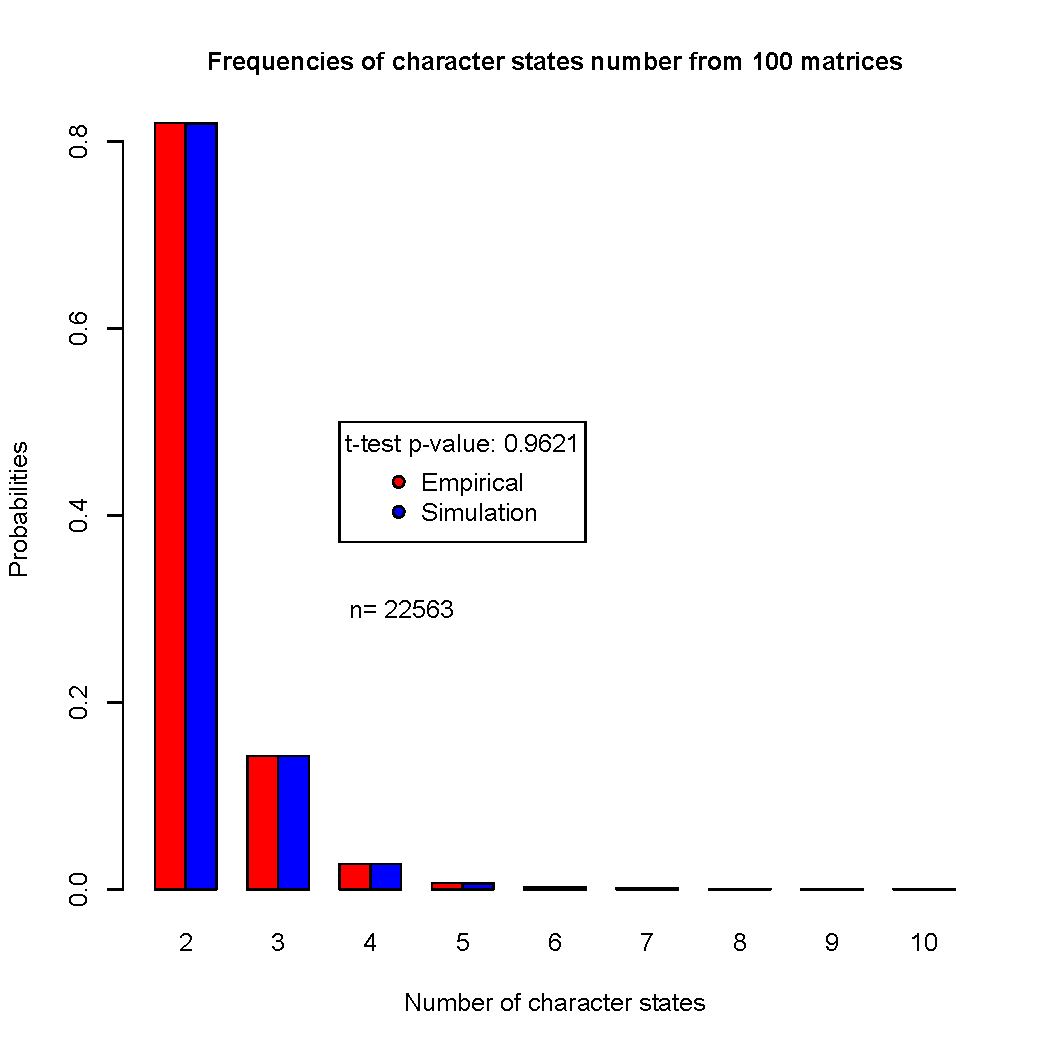
\includegraphics[keepaspectratio=true]{SupplementaryMaterial/Supp_Figures/TEM_Fig-AppendixCharacters.pdf}
\caption{Character states distribution in empirical matrices. %Title?
Characters states number distribution extracted from 100 random morphological matrices downloaded from RreeBase.}
\label{Fig_AppendixCharacters}
\end{figure}


\subsection{Tree Building Software settings}

\subsubsection{Maximum Likelihood - RAxML v8.0.20 \citep{Stamatakis21012014}}

Model: \\
Molecular data: \\
GTR + $\Gamma_4$ (-m GTRGAMMA) \\
Morphological data: \\
Mk + $\Gamma_4$ (-K MK) \\
Support: \\
Rapid Boostrap algorithm (LSR), 1000 replicates \\

\subsubsection{Bayesian - MrBayes v3.2.1 \citep{Ronquist2012mrbayes}}

Priors: \\
Molecular data: \\
rates distribution shape ($\alpha$) = 0.5 \\
Transition/Transversion ratio = 2 ($\beta$(80,40)) \\
Starting tree: "True" tree topology with each branch length = 1 \\
Morphological data: \\
rates distribution shape ($\alpha$) = 0.5 \\
Models: \\
Molecular data: HKY + $\Gamma_4$ \\
Morphological data: Mk + $\Gamma_4$ \\
MCMC: \\
2 runs \\
4 chains per run \\
generations < 50$\times$$1^6$ \\
sample frequency = 1050$\times$$1^3$ \\
ASDS diagnosis frequency = 50$\times$$1^3$ \\
ASDS $<$ 0.01 \\
ESS $>>$ 200 \\
Burnin = 25\%